\documentclass[12pt]{report}
\usepackage[utf8]{inputenc}
\usepackage[russian]{babel}
%\usepackage[14pt]{extsizes}
\usepackage{listings}
\usepackage{graphicx}
\usepackage{amsmath,amsfonts,amssymb,amsthm,mathtools} 
\usepackage{pgfplots}
\usepackage{filecontents}
\usepackage{indentfirst}
\usepackage{eucal}
\usepackage{float}
\usepackage{amsmath}
\usepackage{enumitem}
\frenchspacing

\usepackage{indentfirst} % Красная строка


%\usetikzlibrary{datavisualization}
%\usetikzlibrary{datavisualization.formats.functions}

\usepackage{amsmath}


% Для листинга кода:
\lstset{ %
	language=haskell,                 % выбор языка для подсветки (здесь это С)
	basicstyle=\small\sffamily, % размер и начертание шрифта для подсветки кода
	numbers=left,               % где поставить нумерацию строк (слева\справа)
	numberstyle=\tiny,           % размер шрифта для номеров строк
	stepnumber=1,                   % размер шага между двумя номерами строк
	numbersep=5pt,                % как далеко отстоят номера строк от подсвечиваемого кода
	showspaces=false,            % показывать или нет пробелы специальными отступами
	showstringspaces=false,      % показывать или нет пробелы в строках
	showtabs=false,             % показывать или нет табуляцию в строках
	frame=single,              % рисовать рамку вокруг кода
	tabsize=2,                 % размер табуляции по умолчанию равен 2 пробелам
	captionpos=t,              % позиция заголовка вверху [t] или внизу [b] 
	breaklines=true,           % автоматически переносить строки (да\нет)
	breakatwhitespace=false, % переносить строки только если есть пробел
	escapeinside={\#*}{*)}   % если нужно добавить комментарии в коде
}

\usepackage[left=2cm,right=2cm, top=2cm,bottom=2cm,bindingoffset=0cm]{geometry}
% Для измененных титулов глав:
\usepackage{titlesec, blindtext, color} % подключаем нужные пакеты
\definecolor{gray75}{gray}{0.75} % определяем цвет
\newcommand{\hsp}{\hspace{20pt}} % длина линии в 20pt
% titleformat определяет стиль
\titleformat{\chapter}[hang]{\Huge\bfseries}{\thechapter\hsp\textcolor{gray75}{|}\hsp}{0pt}{\Huge\bfseries}


% plot
\usepackage{pgfplots}
\usepackage{filecontents}
\usetikzlibrary{datavisualization}
\usetikzlibrary{datavisualization.formats.functions}

\begin{document}
	%\def\chaptername{} % убирает "Глава"
	\thispagestyle{empty}
	\begin{titlepage}
		\noindent \begin{minipage}{0.15\textwidth}
			
\includegraphics[width=\linewidth]{b_logo}
		\end{minipage}
		\noindent\begin{minipage}{0.9\textwidth}\centering
			\textbf{Министерство науки и высшего образования Российской Федерации}\\
			\textbf{Федеральное государственное бюджетное образовательное учреждение высшего образования}\\
			\textbf{~~~«Московский государственный технический университет имени Н.Э.~Баумана}\\
			\textbf{(национальный исследовательский университет)»}\\
			\textbf{(МГТУ им. Н.Э.~Баумана)}
		\end{minipage}
		
		\noindent\rule{18cm}{3pt}
		\newline\newline
		\noindent ФАКУЛЬТЕТ $\underline{\text{«Информатика и системы управления»}}$ \newline\newline
		\noindent КАФЕДРА $\underline{\text{«Программное обеспечение ЭВМ и информационные технологии»}}$\newline\newline\newline\newline\newline
		
		
		\begin{center}
			\noindent\begin{minipage}{1.3\textwidth}\centering
				\Large\textbf{  Отчёт по лабораторной работе №7}\newline
				\textbf{по дисциплине "Анализ алгоритмов"}\newline\newline
			\end{minipage}
		\end{center}
		
		\noindent\textbf{Тема} $\underline{\text{Поиск в словаре}}$\newline\newline
		\noindent\textbf{Студент} $\underline{\text{Варламова Е. А.}}$\newline\newline
		\noindent\textbf{Группа} $\underline{\text{ИУ7-51Б}}$\newline\newline
		\noindent\textbf{Преподаватели} $\underline{\text{Волкова Л.Л.}}$\newline\newline\newline
		
		\begin{center}
			\vfill
			Москва~---~\the\year
			~г.
		\end{center}
	\end{titlepage}
	
\setcounter{page}{2}	
	\tableofcontents
	
\newpage
\chapter*{Введение}
\addcontentsline{toc}{chapter}{Введение}
	
Словарь  -- структура данных, построенная  на  основе  пар  значений.  Первое  значение  пары -- ключ  для идентификации элементов, второе  -- собственно сам хранимый элемент. Например, в телефонном справочнике номеру  телефона  соответствует  фамилия  абонента. Задача поиска в слове является очень актуальной в современных системах, так как чаще всего идентификатор не может быть представлен индексом (то есть числовым значением).
	
\section*{Цель лабораторной работы}
	
Целью данной лабораторной работы является разработка эффективного алгоритма поиска в словаре.
	
\section*{Задачи лабораторной работы}
	
В рамках выполнения работы необходимо решить следующие задачи:
	
\begin{itemize}
	\item реализовать три алгоритма поиска в словаре: линейный, двоичный, по сегментам;
	\item оценить трудоёмкости алгоритмов в лучшем случае, худшем случае и в среднем;
	\item провести анализ алгоритмов по количеству сравнений.
\end{itemize}
	
\chapter{Аналитическая часть}
	
В данном разделе представленные теоретические сведения о рассматриваемых алгоритмах.
	
\section{Линейный поиск}
	
Алгоритм линейного поиска заключается в проходе по словарю, до того момента, пока не будет найден искомый ключ. В рассматриваемом алгоритме возможно $N + 1$ случаев расположения ключа: ключ является $i$-ым элементом словаря либо его нет в словаре в принципе. 
	
Лучший случай (трудоемкость $O(1)$): ключ расположен в самом начале словаря и найден за одно сравнение). Худший случай (трудоемкость $O(N)$): ключ расположен в самом конце словаря либо ключ не находится в словаре. Средний случай: $O(N/2) = O(N)$.
	
\section{Двоичный поиск}
	
Данный алгоритм подходит только для заранее упорядоченного словаря.
	
Процесс двоичного поиска можно описать следующим образом: 
	
\begin{itemize}
	\item получить значение находящееся в середине словаря и сравнить его с ключом;
	\item в случае, если ключ меньше данного значения, продолжить поиск в младшей части словаря, в обратном случае -- в старшей части словаря;
	\item на новом интервале снова получить значение из середины этого интервала и сравнить с ключом.
	\item поиск продолжать до тех пор, пока не будет найден искомый ключ, или интервал поиска не окажется пустым.
\end{itemize}
	
Обход словаря данным алгоритм можно представить в виде дерева, поэтому трудоемкость в худшем случае и в среднем составит $\log_{2}{N}$. Трудоёмкость в лучшем случае: $O(1)$ (элемент сразу оказался средним). Можно сделать вывод, что алгоритм двоичного поиска работает значительно быстрее, чем алгоритм линейного поиска, однако при этом он требует предварительной обработки данных (сортировки).
	
\section{Поиск по сегментам}
	
Данный алгоритм также требует предварительной обработки данных, а именно:
\begin{itemize}
	\item упорядочить словарь;
	\item разбить словарь на сегменты.
\end{itemize}
	
Словарь разбивается на сегменты по какому-либу признаку и сортируется по частоте. Например, если ключ является строкой, то можно сделать разбиение по первой букве в ключе. Если ключ является целым числом, можно провести разбиение по остатку от деления ключа на некоторое число $K$.
	
После выполнения разбиения, нужно определить к какому сегменту относится искомый ключ и провести на этом сегменте двоичный поиск.
	
Таким образом, так же, как и алгоритм двоичного поиска, поиск по сегментам требует предварительной обработки данных. 

Трудоёмкость поиска по сегментам складывается из двух величин: трудоёмкости линейного поиска сегмента и бинарного поиска внутри сегмента.
	
\section{Описание словаря}
Словарь представляет собой массив пар (название фильма, год выпуска). Информация взята с портала министерства культуры РФ [1].
	
\section*{Вывод}
В данном разделе были рассмотренны особенности алгоритмов поиска в словаре. Кроме того, бьли приведены трудоёмкости каждого из алгоритмов.
	
\chapter{Конструкторская часть}
	
В данном разделе представлены схемы рассматриваемых алгоритмов.
	
\section{Разработка алгоритмов}
	
На рисунках \ref{fig:s}, \ref{fig:bs} и \ref{fig:ss} приведены схемы алгоритмов поиска в словаре. На рисунке  \ref{fig:seg} приведён алгоритм сегментирования для поиска по сегментам.
	
	\begin{figure}[H]
		\centering
		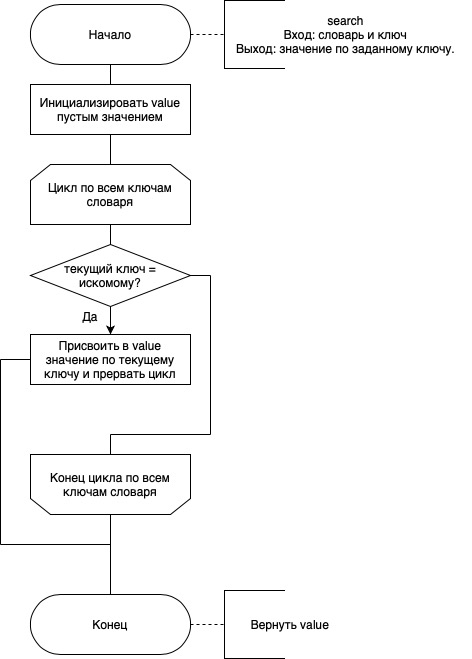
\includegraphics[scale=0.57]{scheme-search.jpg}
		\caption{Схема алгоритма полного перебора.}
		\label{fig:s}
	\end{figure}
	
	\begin{figure}[H]
		\centering
		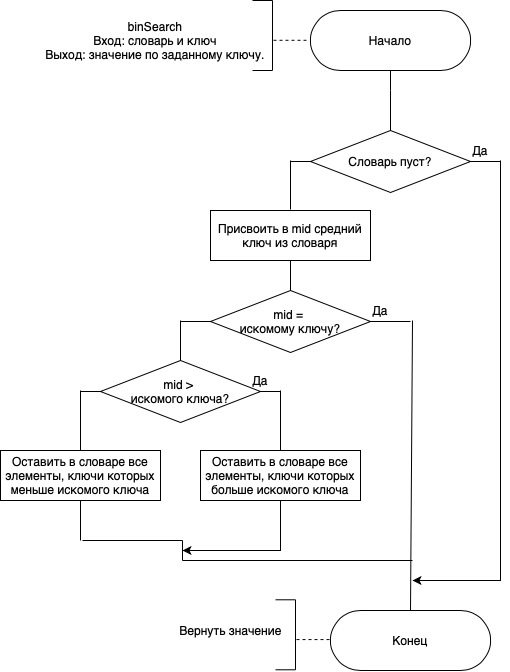
\includegraphics[scale=0.55]{scheme-binSearch.jpg}
		\caption{Схема алгоритма двоичного поиска.}
		\label{fig:bs}
	\end{figure}
	
	\begin{figure}[H]
		\centering
		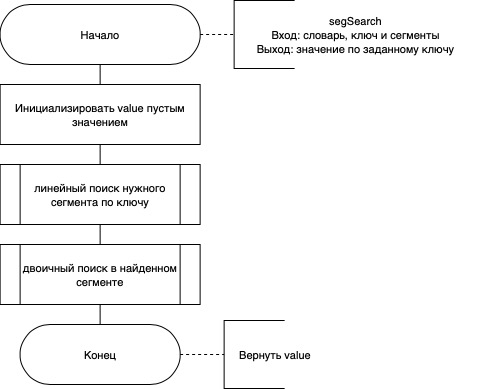
\includegraphics[scale=0.6]{scheme-segSearch.jpg}
		\caption{Схема алгоритма поиска по сегментам.}
		\label{fig:ss}
	\end{figure}

	\begin{figure}[H]
		\centering
		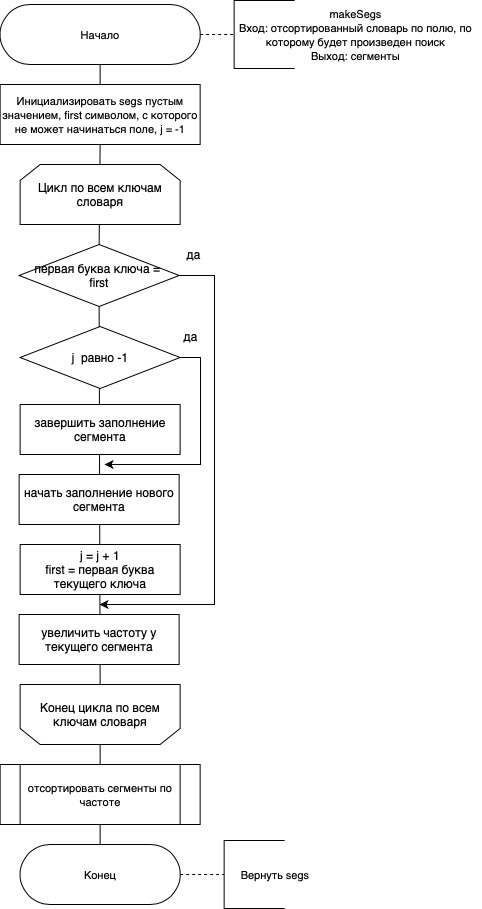
\includegraphics[scale=0.6]{scheme-makeSegs.jpg}
		\caption{Схема алгоритма сегментирования.}
		\label{fig:seg}
	\end{figure}
	
	
	\section*{Вывод}
	
	На основе теоретических данных, полученных аз аналитического раздела, были построенны схемы алгоритмов поиска в словаре. 
	
	\chapter{Технологическая часть}
	
	В данном разделе приведены средства реализации и листинги кода.
	
	\section{Средства реализации}
	
	Для реализации ПО я выбрал язык программирования Python. Данный выбор обусловлен тем, что язык обладает мощными инструментами работы со списками и строками, которые облегчают написание программ. Кроме того, существует множество библиотек для Python [2], в том числе, работа с json [3], matplotlib [4], numpy [5].
	
\section{Реализация алгоритмов}

В листингах \ref{search_code}, \ref{bs_code} и \ref{ss_code} представлены листинги алгоритмов поиска в словаре.
	
\begin{lstlisting}[label=search_code,caption=Алгоритм линейного поиска, language=Python]
def search(d, key, comp):
    for i in range(len(d)):
        if comp(d[i], key) == 0:
            return d[i], i + 1
    return "not found", len(d)
\end{lstlisting}

\begin{lstlisting}[label = bs_code,caption=Алгоритм двоичного поиска, language=Python]
def binSearch(d, key, comp, lo, hi):
    cmp = 0
    while lo < hi:
        cmp += 1
        mid = (lo+hi)//2
        midval = d[mid]
        if comp(midval, key) < 0:
            lo = mid+1
            cmp += 1
        elif comp(midval, key) > 0: 
            hi = mid
            cmp += 2
        else:
            cmp += 2
            return d[mid], cmp
    return "not found", cmp
\end{lstlisting}

\begin{lstlisting}[label=ss_code,caption=Алгоритм поиска по сегментам, language=Python]
def make_segments(d):
    segments = []
    first = '\n'
    j = -1
    d.sort(key = lambda f: f.name)
    for i in range (len(d)):
        if d[i].name[0] != first:
            if j != -1:
                segments[j].end = i - 1
            
            segments.append(Segment(d[i].name[0], i, -1, 1))
            j += 1
            first = d[i].name[0]
        else:
            segments[j].freq += 1
    segments.sort(key = lambda s: s.freq, reverse = True)
    return segments
    
def segSearch(d, segments, key, comp):
    t = search(segments, key.lower()[0], segComp)
    tmp = binSearch(d, key, comp, t[0].beg, t[0].end + 1)
    return tmp[0], t[1] + tmp[1]
\end{lstlisting}
	
\section{Тестовые данные}

В таблице \ref{test_table} приведены тестовые данные, где ЛП -- линейный поиск, ДП -- двоичный поиск, СП - поиск по сегментам. Все тесты были пройденны успешно.

\begin{table}[H]
	\caption{Таблица тестовых данных алгоритмов поиска в словаре.}
	\label{test_table}
	\begin{center}

		\begin{tabular}{|c c c c c|} 

			\hline

			Входные данные & Ожидаемый результат & ЛП & ДП & СП \\  

			\hline

			азартные игры & 1999 & 1999 & 1999 & 1999 \\

			\hline

			супервычислитель & 2013 & 2013 & 2013 & 2013 \\

			\hline

			куприн & 2013 & 2013 & 2013 & 2013 \\

			\hline

			музыка & Нет ключа & Нет ключа & Нет ключа & Нет ключа \\
			\hline
		\end{tabular}

	\end{center}

\end{table}
	
\section*{Вывод}
	
В данном разделе была разработаны и протестированны алгоритмы поиска в словаре. Кроме того, было показано, что алгоритмы двоичного поиска и алгоритм поиска по сегментам требуют предварительный обработки данных (сортировки и разбиение на сегменты соотвественно), в отличие от алгоритма линейного поиска.
	
\chapter{Исследовательская часть}
	
В данном разделе приведен анализ характеристик разработанного ПО.
	
\section{Анализ алгоритмов по количеству сравнений}

На рисунках \ref{fig:lin_sc}, \ref{fig:bin_sc} и \ref{fig:seg_sc} приведены графики линейного, бинарного поиска и поиска по сегментам по количеству сравнений. В таблице 4.1 приведено соотвестсвие индексов названиям фильмов.
	
	\begin{figure}[H]
		\centering
		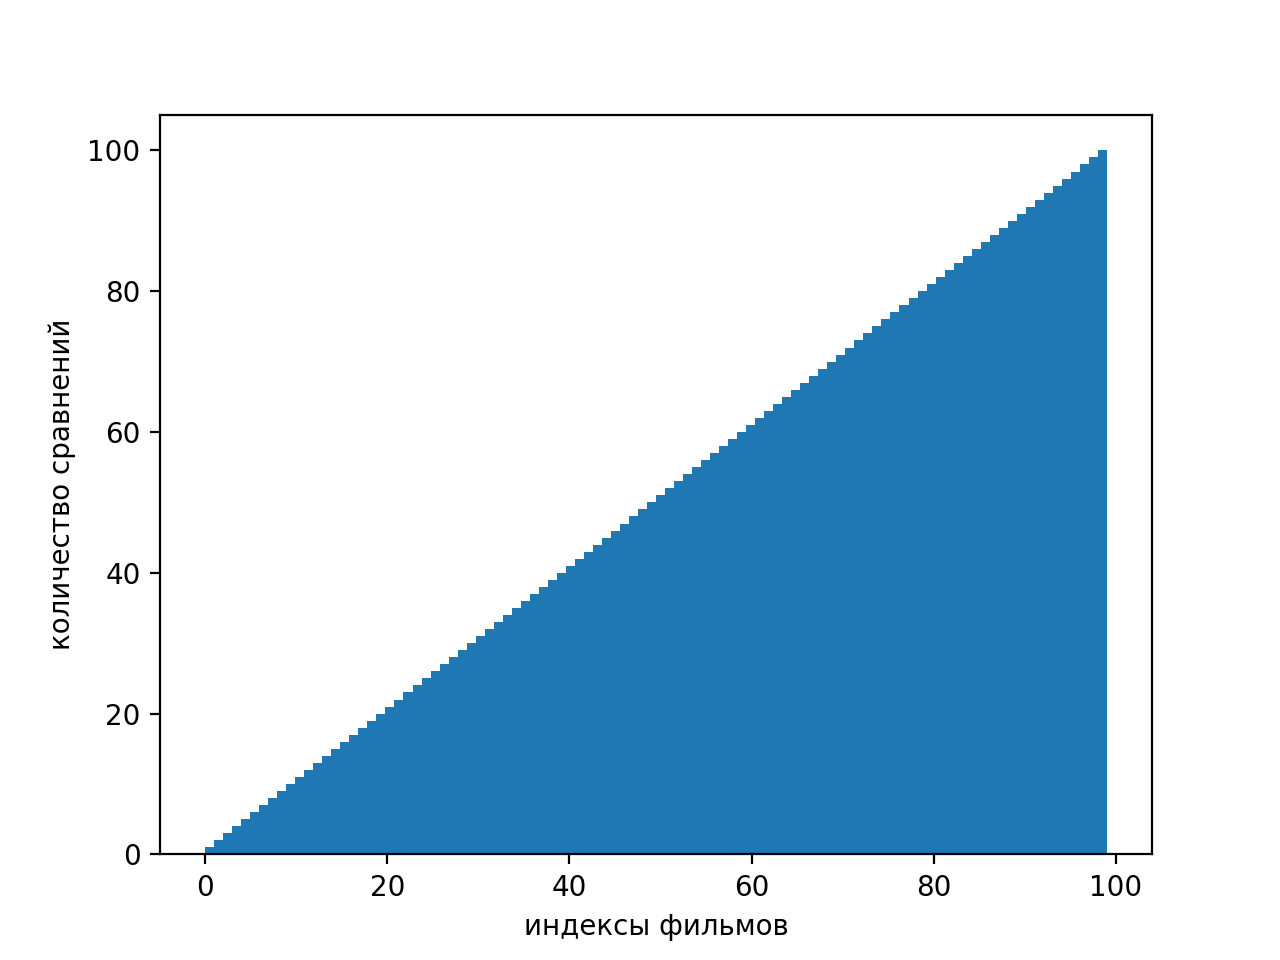
\includegraphics[scale=0.9]{lin.png}
		\caption{График алгоритма линейного поиска.}
		\label{fig:lin_sc}
	\end{figure}
	
		\begin{figure}[H]
		\centering
		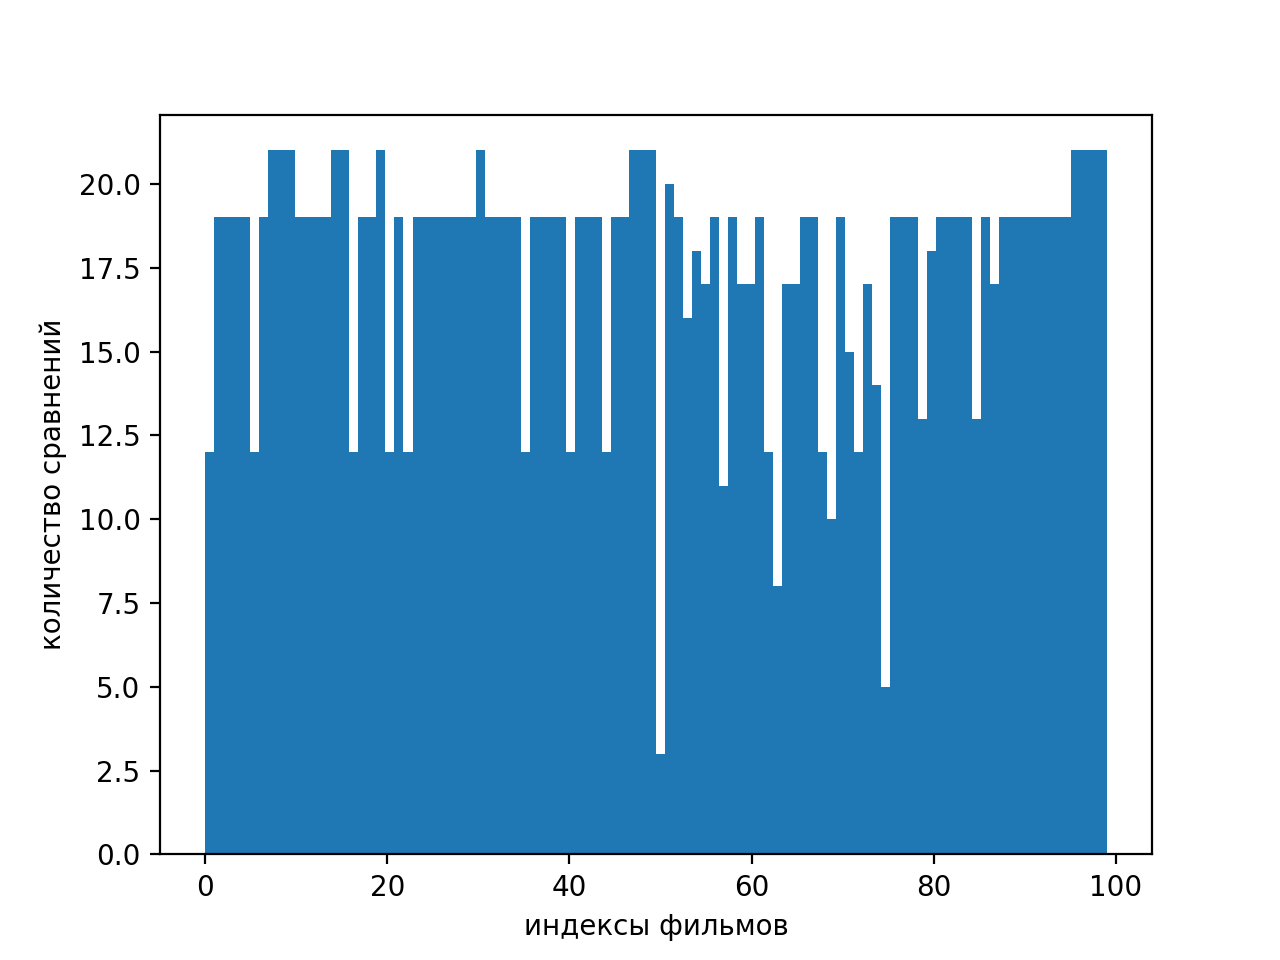
\includegraphics[scale=0.7]{bin.png}
		\caption{График алгоритма бинарного поиска.}
		\label{fig:bin_sc}
	\end{figure}
	
		\begin{figure}[H]
		\centering
		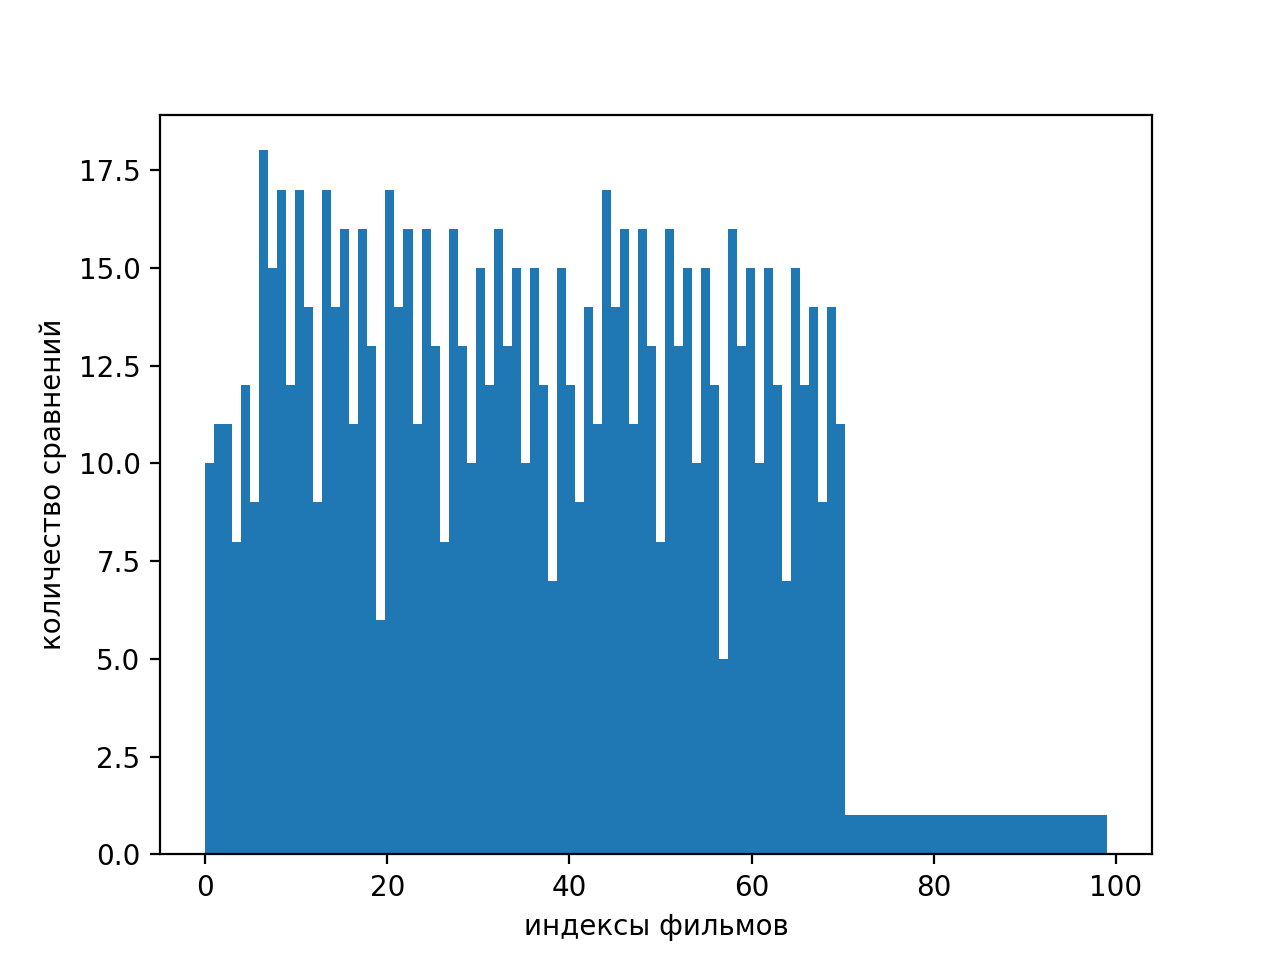
\includegraphics[scale=0.7]{seg.png}
		\caption{График алгоритма поиска по сегментам.}
		\label{fig:seg_sc}
	\end{figure}
	
На рисунках \ref{fig:lin_sc_sorted}, \ref{fig:bin_sc_sorted} и \ref{fig:seg_sc_sorted} приведена та же информация, отсортированная по количеству сравнений. В таблице 4.2 приведено соотвестсвие индексов названиям фильмов.
	
	\begin{figure}[H]
		\centering
		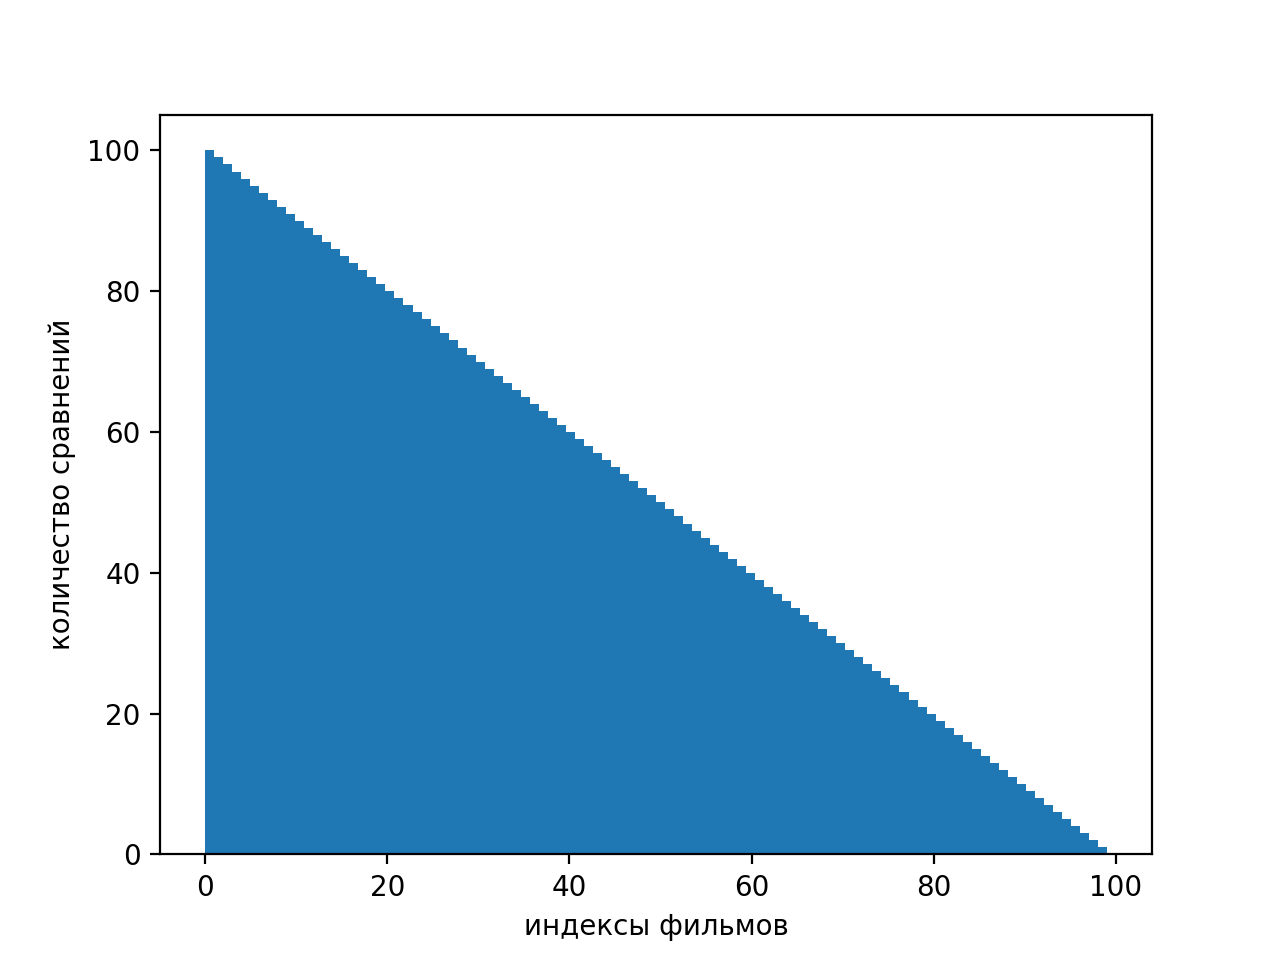
\includegraphics[scale=0.7]{lin_sorted.png}
		\caption{График алгоритма линейного поиска.}
		\label{fig:lin_sc_sorted}
	\end{figure}
	
		\begin{figure}[H]
		\centering
		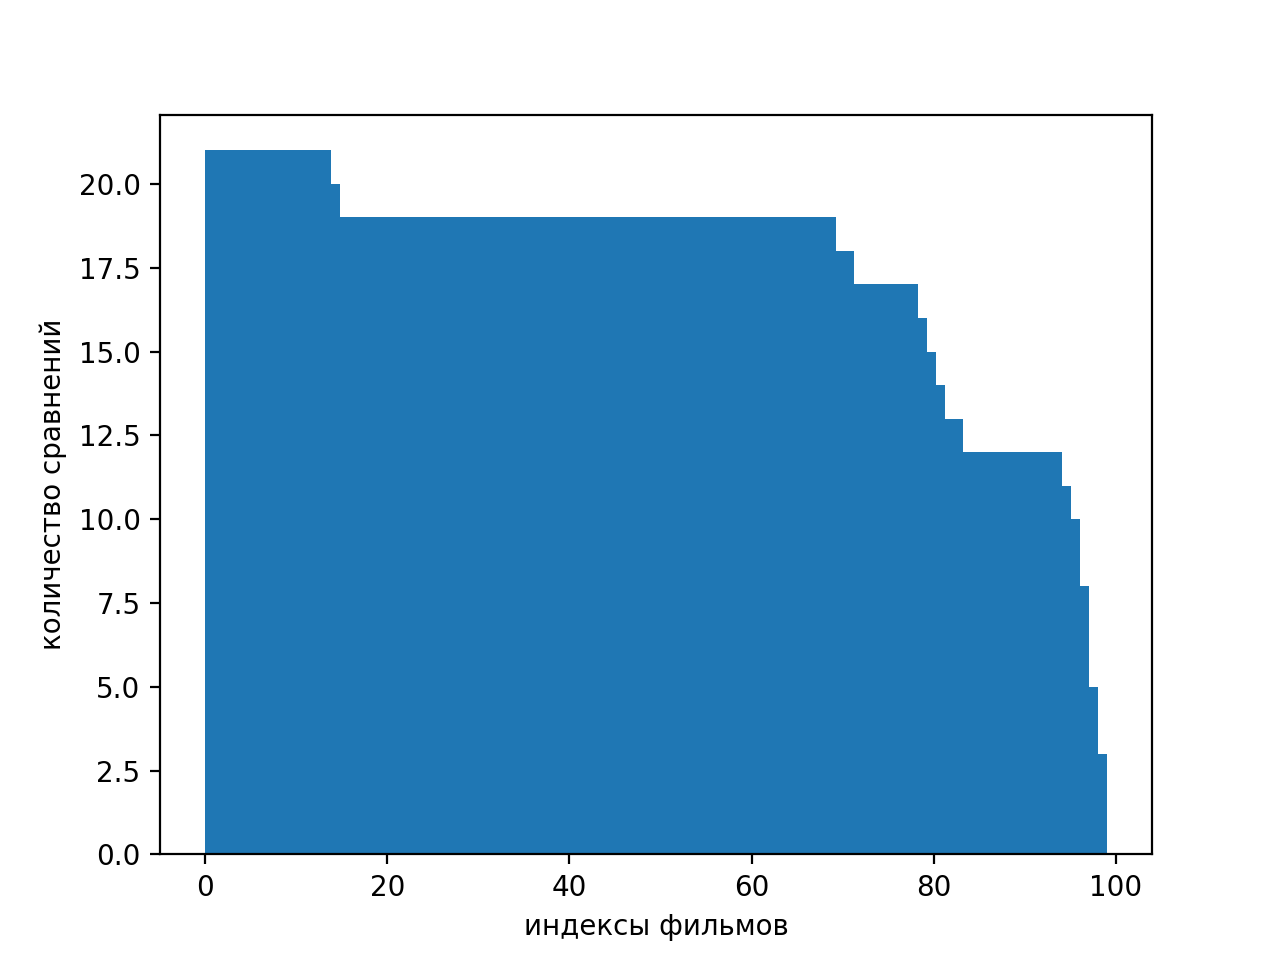
\includegraphics[scale=0.7]{bin_sorted.png}
		\caption{График алгоритма бинарного поиска.}
		\label{fig:bin_sc_sorted}
	\end{figure}
	
		\begin{figure}[H]
		\centering
		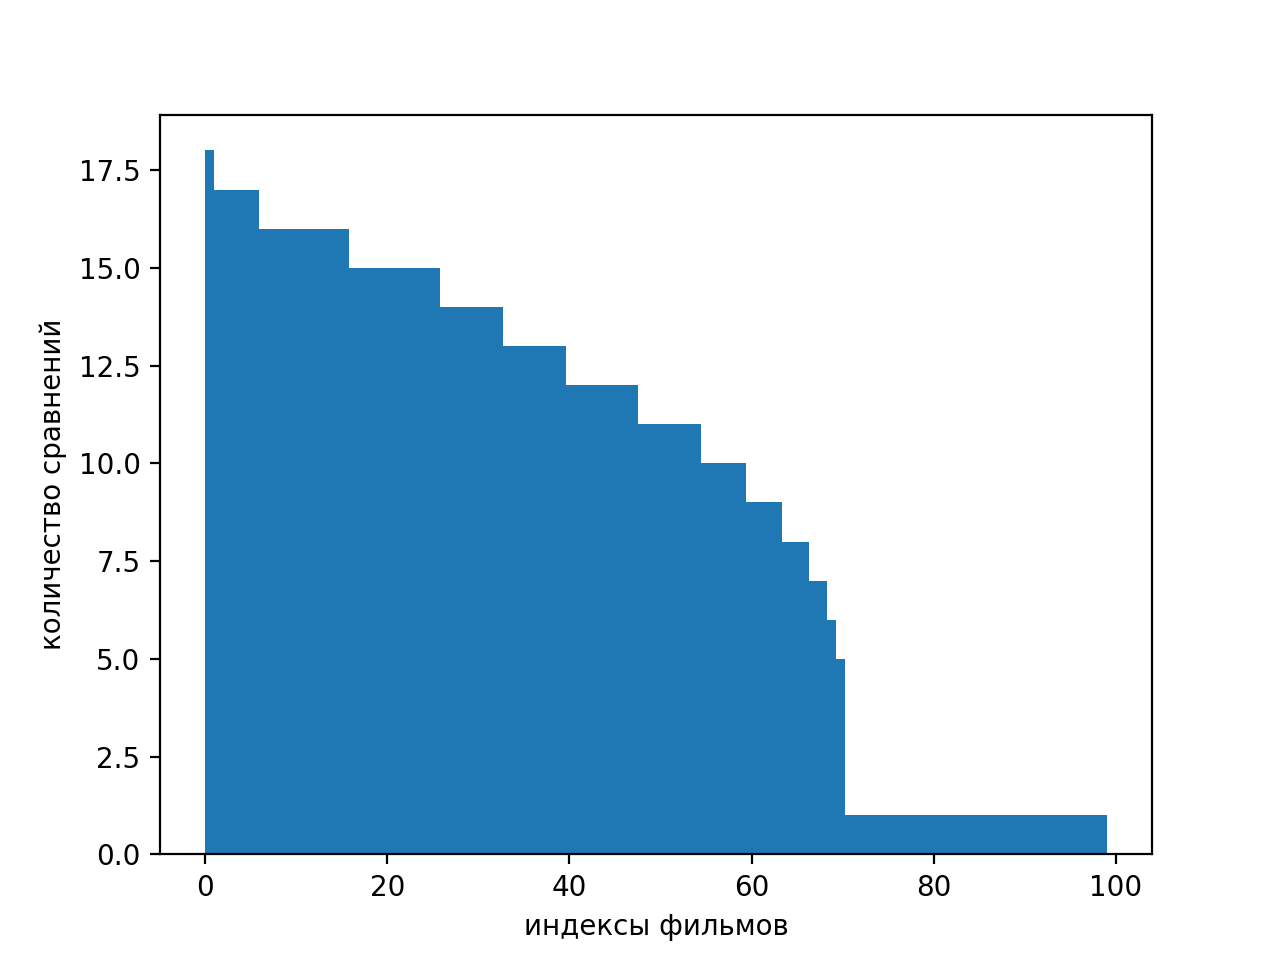
\includegraphics[scale=0.9]{seg_sorted.png}
		\caption{График алгоритма поиска по сегментам.}
		\label{fig:seg_sc_sorted}
	\end{figure}
\begin{table}[H]
	\caption{Соотвествие индексов названиям фильмов (№1)}
	\label{tab:v6}
	\begin{center}

		\begin{tabular}{|c@{\hspace{7mm}}|c@{\hspace{7mm}}|c@{\hspace{7mm}}|c|c|}

			\hline
			индекс        & название фильма    \\
0 & почти знаменит \\
1 & открытое окно. \\
2 & открытый простор \\
3 & особо важное задание \\
4 & особо опасен \\
5 & поющее звенящее деревце \\
6 & остановился поезд \\
7 & любовь и голуби \\
8 & любовь и сигареты \\
9 & маленькая черная книжка \\
10 & от заката до рассвета \\
11 & отпетые мошенники. \\
12 & отпуск без конца \\
13 & отпуск за свой счет \\
14 & маньчжурский вариант \\
15 & марафонец \\
16 & превосходство борна /по одноименной новелле роберта ладлэма/ \\
17 & ответный ход \\
18 & отдаленные последствия \\
19 & малышка на миллион  \\
20 & преданный садовник \\
21 & отель /по мотивам пьесы джона уэбстера/ \\
22 & председатель \\
23 & осенний марафон \\
24 & осенняя соната \\
25 & осень \\
26 & неподдающиеся \\
27 & неподсуден \\
28 & осмозис джонс \\
29 & невиновный \\
30 & малена. \\
31 & нежная кожа \\
32 & незабываемый 1919-й год \\
33 & незаконченная жизнь \\
34 & незваные. \\
35 & приготовьте ваши носовые платки \\
36 & операция "ы" и другие приключения шурика \\
37 & неизвестные страницы из жизни разведчика \\
38 & неисправимый лгун \\
39 & определитель \\
40 & призрак замка моррисвиль \\
41 & неприкасаемые \\
42 & непристойное предложение /по произведению джека энджелхарда/ \\
\hline
		\end{tabular}
	\end{center}
\end{table}
\begin{table}[H]
	\label{tab:v6}
	\begin{center}

		\begin{tabular}{|c@{\hspace{7mm}}|c@{\hspace{7mm}}|c@{\hspace{7mm}}|c|c|}
		\hline
43 & неразгаданное \\
44 & приключения голубого рыцаря \\
45 & орел приземлился /по роману джека хиггинса/ \\
46 & оружейный барон \\
47 & мастера ужаса 2. дитя демона \\
48 & мастера ужаса 2. звуки \\
49 & мастера ужаса 2. право на смерть \\
50 & мастера ужаса 2. семья \\
51 & мастера ужаса 2. слово на букву "в" \\
52 & очень дикие штучки \\
53 & пираты тихого океана \\
54 & парижские тайны. \\
55 & патруль времени \\
56 & охота \\
57 & охота за красным октябрем /по роману тома клэнси/ \\
58 & папаши._ \\
59 & пикник у висячей скалы \\
60 & петля ориона \\
61 & отставной козы барабанщик \\
62 & плохие парни \\
63 & паршивая овца \\
64 & песни родной стороны \\
65 & пиноккио \\
66 & отсчет утопленников \\
67 & охота на зверя \\
68 & плюмбум, или опасная игра \\
69 & первое свидание \\
70 & охота на лис. \\
71 & пиноккио /по повести карло коллоди "приключения пиноккио"/. \\
72 & пиноккио 3000 \\
73 & перелом \\
74 & питер пэн. \\
75 & пленники небес /по книге джеймса ли бэрка/ \\
76 & мишка-мохнатик (мультипликационный сериал) \\
77 & мисс поттер \\
78 & микки: однажды под рождество \\
79 & план игры \\
80 & парк юрского периода \\
81 & миссис хендерсон представляет \\
82 & муза \\
83 & молодой мастер \\
84 & меч в камне \\
85 & планета ка-пэкс /по мотивам романа джин бруэр/ \\
86 & мистер 3000 \\
87 & персона \\
88 & молчание \\
\hline
		\end{tabular}
	\end{center}
\end{table}
\begin{table}[H]
	\label{tab:v6}
	\begin{center}

		\begin{tabular}{|c@{\hspace{7mm}}|c@{\hspace{7mm}}|c@{\hspace{7mm}}|c|c|}
		\hline
89 & молчи в тряпочку \\
90 & молчун. \\
91 & миротворец \\
92 & мужики!.. \\
93 & мечтатель \\
94 & мой принц \\
95 & мертвец \\
96 & аладдин_ \\
97 & 1000 мест, которые стоит посетить. австралия \\
98 & 200 сигарет \\
99 & автомобиль, скрипка и собака клякса \\
\hline
		\end{tabular}
	\end{center}
\end{table}

\begin{table}[H]
	\caption{Соотвествие индексов названиям фильмов (№2)}
	\label{tab:v6}
	\begin{center}

		\begin{tabular}{|c@{\hspace{7mm}}|c@{\hspace{7mm}}|c@{\hspace{7mm}}|c|c|}

			\hline
			индекс        & название фильма    \\
0 & ответный ход \\
1 & отдаленные последствия \\
2 & малышка на миллион  \\
3 & преданный садовник \\
4 & отель /по мотивам пьесы джона уэбстера/ \\
5 & председатель \\
6 & осенний марафон \\
7 & осенняя соната \\
8 & осень \\
9 & неподдающиеся \\
10 & неподсуден \\
11 & осмозис джонс \\
12 & невиновный \\
13 & малена. \\
14 & нежная кожа \\
15 & незабываемый 1919-й год \\
16 & незаконченная жизнь \\
17 & незваные. \\
18 & приготовьте ваши носовые платки \\
19 & операция "ы" и другие приключения шурика \\
20 & неизвестные страницы из жизни разведчика \\
21 & неисправимый лгун \\
22 & определитель \\
23 & призрак замка моррисвиль \\
24 & неприкасаемые \\
25 & непристойное предложение /по произведению джека энджелхарда/ \\
26 & неразгаданное \\
27 & приключения голубого рыцаря \\
28 & орел приземлился /по роману джека хиггинса/ \\
29 & оружейный барон \\
30 & мастера ужаса 2. дитя демона \\
31 & мастера ужаса 2. звуки \\
32 & мастера ужаса 2. право на смерть \\
33 & мастера ужаса 2. семья \\
34 & мастера ужаса 2. слово на букву "в" \\
35 & очень дикие штучки \\
36 & пираты тихого океана \\
37 & парижские тайны. \\
38 & патруль времени \\
39 & охота \\
40 & охота за красным октябрем /по роману тома клэнси/ \\
41 & папаши._ \\
42 & пикник у висячей скалы \\
\hline
		\end{tabular}
	\end{center}
\end{table}
\begin{table}[H]
	\label{tab:v6}
	\begin{center}

		\begin{tabular}{|c@{\hspace{7mm}}|c@{\hspace{7mm}}|c@{\hspace{7mm}}|c|c|}
		\hline
43 & петля ориона \\
44 & отставной козы барабанщик \\
45 & плохие парни \\
46 & паршивая овца \\
47 & песни родной стороны \\
48 & пиноккио \\
49 & отсчет утопленников \\
50 & охота на зверя \\
51 & плюмбум, или опасная игра \\
52 & первое свидание \\
53 & охота на лис. \\
54 & пиноккио /по повести карло коллоди "приключения пиноккио"/. \\
55 & пиноккио 3000 \\
56 & перелом \\
57 & питер пэн. \\
58 & пленники небес /по книге джеймса ли бэрка/ \\
59 & мишка-мохнатик (мультипликационный сериал) \\
60 & мисс поттер \\
61 & микки: однажды под рождество \\
62 & план игры \\
63 & парк юрского периода \\
64 & миссис хендерсон представляет \\
65 & муза \\
66 & молодой мастер \\
67 & меч в камне \\
68 & планета ка-пэкс /по мотивам романа джин бруэр/ \\
69 & мистер 3000 \\
70 & персона \\
71 & молчание \\
72 & молчи в тряпочку \\
73 & молчун. \\
74 & миротворец \\
75 & мужики!.. \\
76 & мечтатель \\
77 & мой принц \\
78 & мертвец \\
79 & аладдин_ \\
80 & 1000 мест, которые стоит посетить. австралия \\
81 & 200 сигарет \\
82 & автомобиль, скрипка и собака клякса \\
83 & алекс и эмма \\
84 & 101 далматинец_ \\
85 & мой лучший любовник \\
86 & меморандум квиллера /по роману адама холла/ \\
87 & мемуары гейши (по роману артура голдена) \\
88 & август раш \\
\hline
		\end{tabular}
	\end{center}
\end{table}
\begin{table}[H]
	\label{tab:v6}
	\begin{center}

		\begin{tabular}{|c@{\hspace{7mm}}|c@{\hspace{7mm}}|c@{\hspace{7mm}}|c|c|}
		\hline
89 & акробат на северном полюсе \\
90 & 15 минут славы \\
91 & балто 2: в поисках волка \\
92 & балто 3: крылья перемен \\
93 & безумно влюбленный \\
94 & аткинс \\
95 & адъютант его превосходительства \\
96 & без свидетелей \\
97 & без солнца \\
98 & 8 мм \\
99 & 88  минут \\
\hline
		\end{tabular}
	\end{center}
\end{table}
\section*{Вывод}
\addcontentsline{toc}{section}{Вывод}	
В результате проведения анализа по количеству сравнений было выяснено, что алгоритм поиска по сегментам использует меньше сравнений, чем бинарный и линейный.

\chapter*{Заключение}
\addcontentsline{toc}{chapter}{Заключение}
	
В рамках данной лабораторной работы лабораторной работы была достигнута её цель: разарботан эффективный алгоритм поиска в словаре. Также выполнены следующие задачи:
\begin{itemize}
	\item реализованы три алгоритма поиска в словаре: линейный, двоичный, по сегментам;
	\item были оценены трудоёмкости алгоритмов в лучшем случае, худшем случае и в среднем;
	\item проведён анализ алгоритмов по количеству сравнений.
\end{itemize}

В результате проведения анализа по количеству сравнений было выяснено, что алгоритм поиска по сегментам использует меньше сравнений, чем бинарный и линейный. При этом стоит отметить, что и алгоритм двоичного поиска, и алгоритм поиска по сегментам требуют предварительный обработки данных (сортировки и разбиение на сегменты соотвественно), в отличие от алгоритма линейного поиска. Но именно это позволяет стать этим алгоритмам намного эффективнее в сравнении с алгоритмом линейного поиска.
\chapter*{Литература}
\addcontentsline{toc}{chapter}{Литература}
\begin{enumerate}
    \item Данные [Электронный ресурс]. Режим доступа: https://opendata.mkrf.ru/opendata. Дата обращения: 10.12.2021.
	\item Документация по языку программирования Python [Электронный ресурс]. Режим доступа: https://docs.python.org/3/index.html. Дата обращения: 10.12.2021.
	    \item Документация по json [Электронный ресурс]. Режим доступа: https://www.json.org/json-en.html. Дата обращения: 10.12.2021.
	\item Документация по matplotlib [Электронный ресурс]. Режим доступа: https://matplotlib.org. Дата обращения: 10.12.2021.
	\item Документация по numpy [Электронный ресурс]. Режим доступа: https://numpy.org. Дата обращения: 10.12.2021.
\end{enumerate}
\end{document}